
% % bare_conf.tex % V1.3 % 2007/01/11 % by Michael Shell % See: %
% http://www.michaelshell.org/ % for current contact information. % % This is a
% skeleton file demonstrating the use of IEEEtran.cls % (requires IEEEtran.cls
% version 1.7 or later) with an IEEE conference paper. % % Support sites: %
% http://www.michaelshell.org/tex/ieeetran/ %
% http://www.ctan.org/tex-archive/macros/latex/contrib/IEEEtran/ % and %
% http://www.ieee.org/

% %************************************************************************* %
% Legal Notice: % This code is offered as-is without any warranty either
% expressed or % implied; without even the implied warranty of MERCHANTABILITY or
% % FITNESS FOR A PARTICULAR PURPOSE! % User assumes all risk. % In no event
% shall IEEE or any contributor to this code be liable for % any damages or
% losses, including, but not limited to, incidental, % consequential, or any
% other damages, resulting from the use or misuse % of any information contained
% here. % % All comments are the opinions of their respective authors and are not
% % necessarily endorsed by the IEEE. % % This work is distributed under the
% LaTeX Project Public License (LPPL) % ( http://www.latex-project.org/ ) version
% 1.3, and may be freely used, % distributed and modified. A copy of the LPPL,
% version 1.3, is included % in the base LaTeX documentation of all distributions
% of LaTeX released % 2003/12/01 or later. % Retain all contribution notices and
% credits. % ** Modified files should be clearly indicated as such, including  **
% % ** renaming them and changing author support contact information. ** % % File
% list of work: IEEEtran.cls, IEEEtran_HOWTO.pdf, bare_adv.tex, %                
%    bare_conf.tex, bare_jrnl.tex, bare_jrnl_compsoc.tex
% %*************************************************************************

% *** Authors should verify (and, if needed, correct) their LaTeX system  *** ***
% with the testflow diagnostic prior to trusting their LaTeX platform *** ***
% with production work. IEEE's font choices can trigger bugs that do  *** *** not
% appear when using other class files.                            *** The
% testflow support page is at: http://www.michaelshell.org/tex/testflow/



% Note that the a4paper option is mainly intended so that authors in countries
% using A4 can easily print to A4 and see how their papers will look in print -
% the typesetting of the document will not typically be affected with changes in
% paper size (but the bottom and side margins will). Use the testflow package
% mentioned above to verify correct handling of both paper sizes by the user's
% LaTeX system.  Also note that the "draftcls" or "draftclsnofoot", not "draft",
% option should be used if it is desired that the figures are to be displayed in
% draft mode.
\documentclass[a4paper,report]{IEEEtran}
% Add the compsoc option for Computer Society conferences.  If IEEEtran.cls has
% not been installed into the LaTeX system files, manually specify the path to it
% like: \documentclass[conference]{../sty/IEEEtran}
 

\usepackage[english]{babel}
\usepackage[utf8]{inputenc}
\usepackage[IL2]{fontenc}


% Some very useful LaTeX packages include: (uncomment the ones you want to load)


% *** MISC UTILITY PACKAGES ***  \usepackage{ifpdf} Heiko Oberdiek's ifpdf.sty is
% very useful if you need conditional compilation based on whether the output is
% pdf or dvi. usage: \ifpdf % pdf code \else % dvi code \fi The latest version of
% ifpdf.sty can be obtained from:
% http://www.ctan.org/tex-archive/macros/latex/contrib/oberdiek/ Also, note that
% IEEEtran.cls V1.7 and later provides a builtin \ifCLASSINFOpdf conditional that
% works the same way. When switching from latex to pdflatex and vice-versa, the
% compiler may have to be run twice to clear warning/error messages.






% *** CITATION PACKAGES ***  \usepackage{cite} cite.sty was written by Donald
% Arseneau V1.6 and later of IEEEtran pre-defines the format of the cite.sty
% package \cite{} output to follow that of IEEE. Loading the cite package will
% result in citation numbers being automatically sorted and properly
% "compressed/ranged". e.g., [1], [9], [2], [7], [5], [6] without using cite.sty
% will become [1], [2], [5]--[7], [9] using cite.sty. cite.sty's \cite will
% automatically add leading space, if needed. Use cite.sty's noadjust option
% (cite.sty V3.8 and later) if you want to turn this off. cite.sty is already
% installed on most LaTeX systems. Be sure and use version 4.0 (2003-05-27) and
% later if using hyperref.sty. cite.sty does not currently provide for
% hyperlinked citations. The latest version can be obtained at:
% http://www.ctan.org/tex-archive/macros/latex/contrib/cite/ The documentation is
% contained in the cite.sty file itself.
\usepackage[T1]{fontenc}




% *** GRAPHICS RELATED PACKAGES ***
\ifCLASSINFOpdf
	
	\usepackage{listings}
	
	\usepackage[pdftex]{graphicx}
	  % declare the path(s) where your graphic files are
	\graphicspath{{../pdf/}{../jpeg/}{../png/}{../eps/}}
	  % and their extensions so you won't have to specify these with every instance
	  % of \includegraphics
	\DeclareGraphicsExtensions{.pdf,.jpeg,.png,.eps}
\else
	\usepackage[dvips]{graphicx}
	\usepackage{listings}
	\graphicspath{{../eps/}}
	\DeclareGraphicsExtensions{.eps}
	
	
	\usepackage{float}
	
	\floatstyle{ruled}
	\newfloat{program}{thp}{lop}
	\floatname{program}{Listing}

  % or other class option (dvipsone, dvipdf, if not using dvips). graphicx will
  % default to the driver specified in the system graphics.cfg if no driver is
  % specified. \usepackage[dvips]{graphicx} declare the path(s) where your
  % graphic files are \graphicspath{{../eps/}} and their extensions so you won't
  % have to specify these with every instance of \includegraphics
  % \DeclareGraphicsExtensions{.eps}
\fi
% graphicx was written by David Carlisle and Sebastian Rahtz. It is required if
% you want graphics, photos, etc. graphicx.sty is already installed on most LaTeX
% systems. The latest version and documentation can be obtained at:
% http://www.ctan.org/tex-archive/macros/latex/required/graphics/ Another good
% source of documentation is "Using Imported Graphics in LaTeX2e" by Keith
% Reckdahl which can be found as epslatex.ps or epslatex.pdf at:
% http://www.ctan.org/tex-archive/info/  latex, and pdflatex in dvi mode, support
% graphics in encapsulated postscript (.eps) format. pdflatex in pdf mode
% supports graphics in .pdf, .jpeg, .png and .mps (metapost) formats. Users
% should ensure that all non-photo figures use a vector format (.eps, .pdf, .mps)
% and not a bitmapped formats (.jpeg, .png). IEEE frowns on bitmapped formats
% which can result in "jaggedy"/blurry rendering of lines and letters as well as
% large increases in file sizes.  You can find documentation about the pdfTeX
% application at: http://www.tug.org/applications/pdftex





% *** MATH PACKAGES ***  \usepackage[cmex10]{amsmath} A popular package from the
% American Mathematical Society that provides many useful and powerful commands
% for dealing with mathematics. If using it, be sure to load this package with
% the cmex10 option to ensure that only type 1 fonts will utilized at all point
% sizes. Without this option, it is possible that some math symbols, particularly
% those within footnotes, will be rendered in bitmap form which will result in a
% document that can not be IEEE Xplore compliant!  Also, note that the amsmath
% package sets \interdisplaylinepenalty to 10000 thus preventing page breaks from
% occurring within multiline equations. Use: \interdisplaylinepenalty=2500 after
% loading amsmath to restore such page breaks as IEEEtran.cls normally does.
% amsmath.sty is already installed on most LaTeX systems. The latest version and
% documentation can be obtained at:
% http://www.ctan.org/tex-archive/macros/latex/required/amslatex/math/


 


% *** SPECIALIZED LIST PACKAGES ***  \usepackage{algorithmic} algorithmic.sty was
% written by Peter Williams and Rogerio Brito. This package provides an
% algorithmic environment fo describing algorithms. You can use the algorithmic
% environment in-text or within a figure environment to provide for a floating
% algorithm. Do NOT use the algorithm floating environment provided by
% algorithm.sty (by the same authors) or algorithm2e.sty (by Christophe Fiorio)
% as IEEE does not use dedicated algorithm float types and packages that provide
% these will not provide correct IEEE style captions. The latest version and
% documentation of algorithmic.sty can be obtained at:
% http://www.ctan.org/tex-archive/macros/latex/contrib/algorithms/ There is also
% a support site at: http://algorithms.berlios.de/index.html Also of interest may
% be the (relatively newer and more customizable) algorithmicx.sty package by
% Szasz Janos: http://www.ctan.org/tex-archive/macros/latex/contrib/algorithmicx/




% *** ALIGNMENT PACKAGES ***  \usepackage{array} Frank Mittelbach's and David
% Carlisle's array.sty patches and improves the standard LaTeX2e array and
% tabular environments to provide better appearance and additional user controls.
% As the default LaTeX2e table generation code is lacking to the point of almost
% being broken with respect to the quality of the end results, all users are
% strongly advised to use an enhanced (at the very least that provided by
% array.sty) set of table tools. array.sty is already installed on most systems.
% The latest version and documentation can be obtained at:
% http://www.ctan.org/tex-archive/macros/latex/required/tools/


% \usepackage{mdwmath} \usepackage{mdwtab} Also highly recommended is Mark
% Wooding's extremely powerful MDW tools, especially mdwmath.sty and mdwtab.sty
% which are used to format equations and tables, respectively. The MDWtools set
% is already installed on most LaTeX systems. The lastest version and
% documentation is available at:
% http://www.ctan.org/tex-archive/macros/latex/contrib/mdwtools/


% IEEEtran contains the IEEEeqnarray family of commands that can be used to
% generate multiline equations as well as matrices, tables, etc., of high
% quality.


% \usepackage{eqparbox} Also of notable interest is Scott Pakin's eqparbox
% package for creating (automatically sized) equal width boxes - aka "natural
% width parboxes". Available at:
% http://www.ctan.org/tex-archive/macros/latex/contrib/eqparbox/





% *** SUBFIGURE PACKAGES *** \usepackage[tight,footnotesize]{subfigure}
% subfigure.sty was written by Steven Douglas Cochran. This package makes it easy
% to put subfigures in your figures. e.g., "Figure 1a and 1b". For IEEE work, it
% is a good idea to load it with the tight package option to reduce the amount of
% white space around the subfigures. subfigure.sty is already installed on most
% LaTeX systems. The latest version and documentation can be obtained at:
% http://www.ctan.org/tex-archive/obsolete/macros/latex/contrib/subfigure/
% subfigure.sty has been superceeded by subfig.sty.



% \usepackage[caption=false]{caption} \usepackage[font=footnotesize]{subfig}
% subfig.sty, also written by Steven Douglas Cochran, is the modern replacement
% for subfigure.sty. However, subfig.sty requires and automatically loads Axel
% Sommerfeldt's caption.sty which will override IEEEtran.cls handling of captions
% and this will result in nonIEEE style figure/table captions. To prevent this
% problem, be sure and preload caption.sty with its "caption=false" package
% option. This is will preserve IEEEtran.cls handing of captions. Version 1.3
% (2005/06/28) and later (recommended due to many improvements over 1.2) of
% subfig.sty supports the caption=false option directly:
% \usepackage[caption=false,font=footnotesize]{subfig}  The latest version and
% documentation can be obtained at:
% http://www.ctan.org/tex-archive/macros/latex/contrib/subfig/ The latest version
% and documentation of caption.sty can be obtained at:
% http://www.ctan.org/tex-archive/macros/latex/contrib/caption/

 


% *** FLOAT PACKAGES ***  \usepackage{fixltx2e} fixltx2e, the successor to the
% earlier fix2col.sty, was written by Frank Mittelbach and David Carlisle. This
% package corrects a few problems in the LaTeX2e kernel, the most notable of
% which is that in current LaTeX2e releases, the ordering of single and double
% column floats is not guaranteed to be preserved. Thus, an unpatched LaTeX2e can
% allow a single column figure to be placed prior to an earlier double column
% figure. The latest version and documentation can be found at:
% http://www.ctan.org/tex-archive/macros/latex/base/



% \usepackage{stfloats} stfloats.sty was written by Sigitas Tolusis. This package
% gives LaTeX2e the ability to do double column floats at the bottom of the page
% as well as the top. (e.g., "\begin{figure*}[!b]" is not normally possible in
% LaTeX2e). It also provides a command: \fnbelowfloat to enable the placement of
% footnotes below bottom floats (the standard LaTeX2e kernel puts them above
% bottom floats). This is an invasive package which rewrites many portions of the
% LaTeX2e float routines. It may not work with other packages that modify the
% LaTeX2e float routines. The latest version and documentation can be obtained
% at: http://www.ctan.org/tex-archive/macros/latex/contrib/sttools/ Documentation
% is contained in the stfloats.sty comments as well as in the presfull.pdf file.
% Do not use the stfloats baselinefloat ability as IEEE does not allow
% \baselineskip to stretch. Authors submitting work to the IEEE should note that
% IEEE rarely uses double column equations and that authors should try to avoid
% such use. Do not be tempted to use the cuted.sty or midfloat.sty packages (also
% by Sigitas Tolusis) as IEEE does not format its papers in such ways.

	\usepackage{tabularx}





% *** PDF, URL AND HYPERLINK PACKAGES ***  \usepackage{url} url.sty was written
% by Donald Arseneau. It provides better support for handling and breaking URLs.
% url.sty is already installed on most LaTeX systems. The latest version can be
% obtained at: http://www.ctan.org/tex-archive/macros/latex/contrib/misc/ Read
% the url.sty source comments for usage information. Basically,
% \url{my_url_here}.





% *** Do not adjust lengths that control margins, column widths, etc. *** *** Do
% not use packages that alter fonts (such as pslatex).         *** There should
% be no need to do such things with IEEEtran.cls V1.6 and later. (Unless
% specifically asked to do so by the journal or conference you plan to submit to,
% of course. )

\def\IEEEkeywordsname{Keywords}
% correct bad hyphenation here
\hyphenation{}

\newcommand{\fig}[1]{Obr.~\ref{fig:#1}}      % abstract for figures

\newcommand{\Sec}[1]{Section~\ref{sec:#1}}  

\newcommand{\listing}[1]{Listing~\ref{listing:#1}}  

\newcommand{\tab}[1]{Table~\ref{tab:#1}}      % abstract for figures


\begin{document}
%  paper title can use linebreaks \\ within to get better formatting as desired
\title{Particle based fluid simulation on GPU}


% author names and affiliations use a multiple column layout for up to three
% different affiliations
\author{\IEEEauthorblockN{Aleš Koblížek}\\
\IEEEauthorblockA{koblial2@fel.cvut.cz}}
 
% conference papers do not typically use \thanks and this command is locked out
% in conference mode. If really needed, such as for the acknowledgment of grants,
% issue a \IEEEoverridecommandlockouts after \documentclass

% for over three affiliations, or if they all won't fit within the width of the
% page, use this alternative format:  \author{\IEEEauthorblockN{Michael
% Shell\IEEEauthorrefmark{1}, Homer Simpson\IEEEauthorrefmark{2}, James
% Kirk\IEEEauthorrefmark{3}, Montgomery Scott\IEEEauthorrefmark{3} and Eldon
% Tyrell\IEEEauthorrefmark{4}}
%\IEEEauthorblockA{\IEEEauthorrefmark{1}School of Electrical and Computer Engineering\\
% Georgia Institute of Technology, Atlanta, Georgia 30332--0250\\ Email: see
% http://www.michaelshell.org/contact.html}
%\IEEEauthorblockA{\IEEEauthorrefmark{2}Twentieth Century Fox, Springfield, USA\\
% Email: homer@thesimpsons.com}
%\IEEEauthorblockA{\IEEEauthorrefmark{3}Starfleet Academy, San Francisco, California 96678-2391\\
% Telephone: (800) 555--1212, Fax: (888) 555--1212}
% \IEEEauthorblockA{\IEEEauthorrefmark{4}Tyrell Inc., 123 Replicant Street, Los
% Angeles, California 90210--4321}}

% use for special paper notices \IEEEspecialpapernotice{(Invited Paper)}
 \IEEEspecialpapernotice{Final report for B4M39GPU course\\winter term 2019/2020}


% make the title area
\maketitle


\begin{abstract}
	There are two basic approaches to simulation of fluid dynamics: Eulerian -- focusing on motion at specific location and Lagrangian -- focusing on motion of individual fluid parcels. This paper focuses on the latter approach. The SPH (Smoothed particle hydrodynamics) computation method has been implemented in compute shader along with OpenGL visualization of the particles. A regular grid is used to accelerate the search for nearest neighbour particles.

\end{abstract}
% IEEEtran.cls defaults to using nonbold math in the Abstract.
% This preserves the distinction between vectors and scalars. However,
% if the conference you are submitting to favors bold math in the abstract,
% then you can use LaTeX's standard command \boldmath at the very start
% of the abstract to achieve this. Many IEEE journals/conferences frown on
% math in the abstract anyway.


% no keywords
%\begin{IEEEkeywords}
%\begin{center}
%Generating Clouds, Cell automata, CUDA, C++, OpenGL, Particles, Billboards,
%AntTweakBar, Glut, Curand, Náhodná čísla na GPU
%\end{center}
%\end{IEEEkeywords}


% For peer review papers, you can put extra information on the cover
% page as needed:
% \ifCLASSOPTIONpeerreview
% \begin{center} \bfseries EDICS Category: 3-BBND \end{center}
% \fi
%
% For peerreview papers, this IEEEtran command inserts a page break and
% creates the second title. It will be ignored for other modes.
\IEEEpeerreviewmaketitle
 
\section{Introduction}
% no \IEEEPARstart
Fluids are very common in various real-world environments, therefore they should not be missing in their virtual counterparts to look realistic. To look realistic, however, a large number of particles is necessary to provide sufficient detail. Since there are no dependencies between the particles, their state can be updated independently in every step, which makes this task perfect for parallelization. 

%\begin{figure}[!h]
%\centering
%\includegraphics[width=2in]{hierarchy}
%\caption{Class hierarchy of the application.}
%\label{fig:hierarchy}
%\end{figure}

\section{Smoothed particle hydrodynamics}
Smoothed particle hydrodynamics is an approach introduced by Monaghan \cite{Articles:Monaghan}.
Each particle $i$ has constant mass $m_{i}$ and rest density $\rho_{0i}$ assigned according to the type of liquid. The particles form a density field

\begin{equation}
	\rho(\mathbf{r}) = \sum_{i} m_{i}W_d(\mathbf{r}-\mathbf{r}_i, h)
\end{equation}

which does not have to be bounded. $W_d$ is a density kernel, it will be explained in the next section along with the other kernels. This density field generates forces $\mathbf{f}_{i}^{pressure}$, $\mathbf{f}_{i}^{viscosity}$ acting on the particles. 

The simulation loop first computes the values of the density field at location of each particle and the force acting on each particle

\begin{equation}
	\mathbf{f}_i = \mathbf{f}_{i}^{pressure} + \mathbf{f}_{i}^{viscosity} + \mathbf{f}_{i}^{external},
\end{equation}

where 

\begin{equation}
	\mathbf{f}_{i}^{viscosity} = \mu\sum_{j}m_j\frac{\mathbf{v}_j-\mathbf{v}_i}{\rho(\mathbf{r}_j)} W_v(\mathbf{r}_i-\mathbf{r}_j, h)
\end{equation}

\begin{equation}
	\mathbf{f}_{i}^{pressure} = -\sum_{j}m_j\frac{p(\mathbf{r}_i)+p(\mathbf{r}_j)}{2\rho(\mathbf{r}_j)} \mathbf{W}_p(\mathbf{r}_i-\mathbf{r}_j, h)
\end{equation}

and $\mathbf{f}_{i}^{external}$ may be collision forces from other objects, gravity, or forces caused by user interaction. $\mu$ is the viscosity coefficient and 

\begin{equation}
	p(\mathbf{r}_i) = k(\rho(\mathbf{r}_i)-\rho_{0i}),
\end{equation}

is the pressure at the location of the particle. $k$ is the pressure coefficient. The particle position is then updated from its velocity 

\begin{equation}
	\mathbf{r}_i = \mathbf{r}_i + s\mathbf{v}_i,
\end{equation}

$s$ being the simulation step. The last step is to update the velocity from the previously computed forces

\begin{equation}
	\mathbf{v}_i = \mathbf{v}_i + s\mathbf{a}_i,
\end{equation}

$\mathbf{a}_i$ is acceleration of the particle computed as

\begin{equation}
	\mathbf{a}_i = \frac{\mathbf{f}_{i}}{\rho(\mathbf{r}_{i})}.
\end{equation}

Morris \cite{Articles:Morris} proposed to add a surface tension force, which should help to maintain sharp interfaces between fluids.

\subsection{Smoothing kernels}
Müller \cite{Articles:Muller} proposed the following kernel to be used for computation of density 

\begin{equation}
	W_d(\mathbf{r},h) = \frac{315}{64\pi h^9}
	\left\{
		\begin{array}{ll}
			(h^2-r^2)^3 	& 0\leq r \leq h\\
			0 						& otherwise
		\end{array}
		\right.
\end{equation}

Its advantage is that there is no square root in the distance computation. The next kernel is used for presure computation

\begin{equation}
	\mathbf{W}_p(\mathbf{r},h) = \frac{\mathbf{r}}{|\mathbf{r}|} \frac{45}{\pi h^6} (h-|\mathbf{r}|)^2
\end{equation}

and the last kernel -- for computation of viscosity
\begin{equation}
	W_v(\mathbf{r},h) = \frac{45}{\pi h^6} (h-|\mathbf{r}|)
\end{equation}

\section{Nearest neighbour search}
The complexity of the SPH algorithm as described above is $O(n^2)$. But a particle is going to be affected only be those particles that are very close to it. Therefore it is possible to reduce computation when computing the density and forces by including only the particles which are near enough. These can be found faster by building an auxilliary data structure before each update step of the particles.

First all the particles are wrapped in a bounding cube, which is partitioned into cells by a uniform square grid. Then a list of particles for each cell is created. The following two methods described by Green \cite{Articles:Green} can be used on a GPU. This paper uses the second one.

\begin{figure*}
	\begin{minipage}{0.25\linewidth}
		\centering
		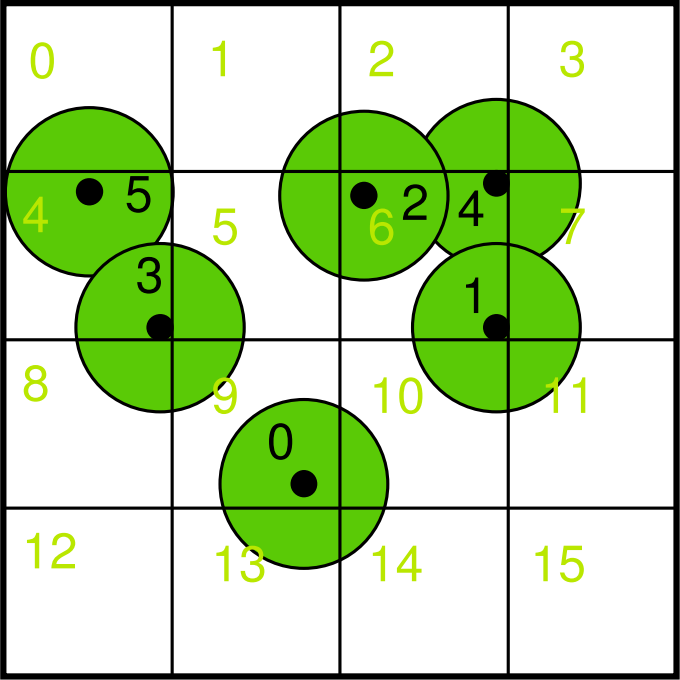
\includegraphics[width=1\linewidth]{grid}
		\caption{Particles in a grid. The green circle marks area with potential neighbours affecting the particle. From \cite{Articles:Green}.}
		\label{fig:grid}
\end{minipage}\hfill
\begin{minipage}{0.7\linewidth}
    \centering

		\begin{tabularx}{1\linewidth}{|c||X|X||X|}
			\hline
			 & Particle records unsorted \newline ($cellID$, $particleID$) & Particle records \newline sorted by $cellID$ & cell records \newline $(firstParticle, N)$ \\
			\hline
			\hline
			0 & (9,0) & (4,3) & (-,0) \\
			1 & (6,1) & (4,5) & (-,0) \\
			2 & (6,2) & (6,1) & (-,0) \\
			3 & (4,3) & (6,2) & (-,0) \\
			4 & (6,4) & (6,4) & (0,2) \\
			5 & (4,5) & (9,0) & (-,0) \\
			6 &       &       & (2,3) \\
			7 &       &       & \dots \\
			\hline
		\end{tabularx}
		\caption{Creating the cell records by sorting the particle records.}
		\label{fig:gridTable}
	\end{minipage}
\end{figure*}

\subsection{Atomic operations}
This approach uses for each cell a counter that stores the number of particles and a fixed-size list of particle indices lying in that cell. Updating the data structure is done with one thread per particle. The thread increments the counter and adds the particle index to the list. This causes scattered writes (and later scattered reads in the particle update phase) and potential bank conflicts.

\subsection{Sorting}
First a list a particle records needs to be built. Each record contains the $cellID$ of the cell it lies in and a $particleID$. These records are then sorted by $cellID$. Then a list of cell records is built, each cell record contains ID of the first particle and number of particles. See figure \ref{fig:grid} and \ref{fig:gridTable}. Finally, the particles are reordered according to the order of particle records. In the update phase, a particle is affected only by particles from the same cell and the cells surrounding it (27 cells in total = $3^3$). 

The size of the cell should be at most $h$, which is the radius of the kernel, because the weight for any particle that is farther away than $h$ will be 0. The $cellID$ can be calculated from 3D coordinates of the particle by first calculating the cell coordinates as 

\begin{equation}
	\mathbf{cell}(\mathbf{r}) = s\frac{\mathbf{r}-\mathbf{BB}_{min}}{\mathbf{BB}_{max} - \mathbf{BB}_{min}}.
\end{equation}

The cell index is then calculated from cell coordinates as

\begin{equation}
	cellID(\mathbf{c}) = c_1s^2 + c_2s + c_3.
\end{equation}

\section{Parallelization}
At the beginning of every frame, the auxilliary data structure must be built. It consists of several steps, which need to be done one after another -- without overlap.
\begin{enumerate}
	\item Create particle records. (parallel)
	\item Sort particle records. (parallel -- using bitonic sort -- see below)
	\item Create cell records. (single thread on GPU)
	\item Reorder particle positions and velocities. (parallel -- different source and destination buffers)
\end{enumerate}
Then the particle positions and velocities can be updated in the following non-overlapping steps.
\begin{enumerate}
	\item Compute density at position of each particle. (parallel)
	\item Update particle positions and velocities. (parallel)
\end{enumerate}

\subsection{Bitonic mergesort}
Bitonic sort is a parallel sorting algorithm based on merging two sorted sequences (a bitonic sequence) into a single one. A bitonic sequence is a sequence that can be split into two sorted sequences, or its circular shift. Figure \ref{fig:bitonicSort} shows a bitonic sorting network. The comparisons and swaps in single column of the red boxes can be executed in parallel. Afterwards, all threads must be synchronized. Therefore this column will correspond to a single compute shader dispatch. Listing \ref{alg:bitonicSort} demonstrates this. Iteration of the inner for loop corresponds to the red-box column within the blue/green-box column, iteration of the outer for loop corresponds to the blue/green-box column in the figure \ref{fig:bitonicSort}.
\begin{figure*}[!h]
\centering
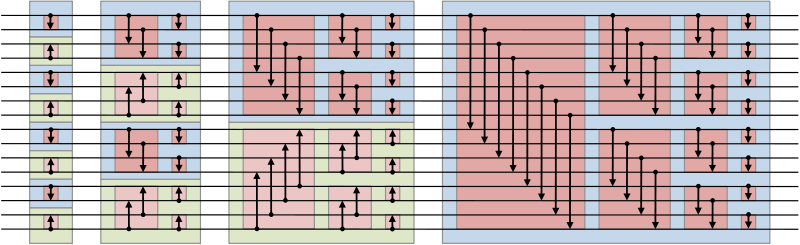
\includegraphics[width=\textwidth]{BitonicSort}
\caption{Bitonic sorting net. The elements to be sorted enter on the wires from the left and exit on the right in a sorted sequence. Arrows represent a comparison between two elements and conditional swap so that the arrow always points to the larger element. On the input of a blue/green block is always a bitonic sequence and on the output is a sorted sequence. Therefore the output of neighbouring blue and green box forms a bitonic sequence, which becomes an input for the next box. From Wikipedia.}
\label{fig:bitonicSort}
\end{figure*}

\lstset{language=C++,caption=Calls to the bitonic sort kernel,frame=single,label=alg:bitonicSort,captionpos=b,basicstyle= \footnotesize,tabsize=1} 
\begin{lstlisting}
	for(size_t b=2; b<2*ParticleN; b*=2) {
		for(size_t seqLen=b; seqLen>1; seqLen/=2) {
			glDispatchCompute(ParticleN/tGroupSize,1,1);
			glMemoryBarrier(...);
		}
	}
\end{lstlisting} 

\section{Implementation details -- compute shaders}
kernel sequence, grid sizes (and reasoning), shm

\section{User interface}

\begin{figure}[!h]
\centering
\includegraphics[width=3in]{screenShotOne}
\caption{Screenshot from the application for TODO particles.}
\label{fig:screenOne}
\end{figure}

\section{Parameter choice and testing}
The SPH method has several parameters. The currently used setting has been determined empirically: TODO. The application was tested visually with these parameters for varying number of particles and NN grid resolution. Particles occasionally get stuck on the boundary due to TODO. Also because the step size is constant and relatively large, the particle never stop moving.

\section{Performance}
table of results for both configurations
commentary (not / as expected, why)

The measured results were obtained on the following configurations:

\begin{itemize}
	\item{Debian 11 GNU/Linux 4.19.0-6-amd64}
	\item{Intel(R) Core(TM) i5-3230M CPU @ 2.60GHz}
	\item{6.0 GB RAM}
	\item{NVIDIA GeForce GT 750M (GK107M)}
	\item{OpenGL Driver version 4.6.0}
	\item{NVIDIA proprietary driver version 418.74}
	\item{384 CUDA cores, 2 GB VRAM}
\end{itemize}


\section{Conclusion}
evaluate results, conclusion, possible improvements



% An example of a floating figure using the graphicx package.
% Note that \label must occur AFTER (or within) \caption.
% For figures, \caption should occur after the \includegraphics.
% Note that IEEEtran v1.7 and later has special internal code that
% is designed to preserve the operation of \label within \caption
% even when the captionsoff option is in effect. However, because
% of issues like this, it may be the safest practice to put all your
% \label just after \caption rather than within \caption{}.
%
% Reminder: the "draftcls" or "draftclsnofoot", not "draft", class
% option should be used if it is desired that the figures are to be
% displayed while in draft mode.
%
%\begin{figure}[!t]
%\centering
%\includegraphics[width=2.5in]{myfigure}
% where an .eps filename suffix will be assumed under latex, 
% and a .pdf suffix will be assumed for pdflatex; or what has been declared
% via \DeclareGraphicsExtensions.
%\caption{Simulation Results}
%\label{fig_sim}
%\end{figure}

% Note that IEEE typically puts floats only at the top, even when this
% results in a large percentage of a column being occupied by floats.


% An example of a double column floating figure using two subfigures.
% (The subfig.sty package must be loaded for this to work.)
% The subfigure \label commands are set within each subfloat command, the
% \label for the overall figure must come after \caption.
% \hfil must be used as a separator to get equal spacing.
% The subfigure.sty package works much the same way, except \subfigure is
% used instead of \subfloat.
%
%\begin{figure*}[!t]
%\centerline{\subfloat[Case I]\includegraphics[width=2.5in]{subfigcase1}%
%\label{fig_first_case}}
%\hfil
%\subfloat[Case II]{\includegraphics[width=2.5in]{subfigcase2}%
%\label{fig_second_case}}}
%\caption{Simulation results}
%\label{fig_sim}
%\end{figure*}
%
% Note that often IEEE papers with subfigures do not employ subfigure
% captions (using the optional argument to \subfloat), but instead will
% reference/describe all of them (a), (b), etc., within the main caption.


% An example of a floating table. Note that, for IEEE style tables, the 
% \caption command should come BEFORE the table. Table text will default to
% \footnotesize as IEEE normally uses this smaller font for tables.
% The \label must come after \caption as always.
%
%\begin{table}[!t]
%% increase table row spacing, adjust to taste
%\renewcommand{\arraystretch}{1.3}
% if using array.sty, it might be a good idea to tweak the value of
% \extrarowheight as needed to properly center the text within the cells
%\caption{An Example of a Table}
%\label{table_example}
%\centering
%% Some packages, such as MDW tools, offer better commands for making tables
%% than the plain LaTeX2e tabular which is used here.
%\begin{tabular}{|c||c|}
%\hline
%One & Two\\
%\hline
%Three & Four\\
%\hline
%\end{tabular}
%\end{table}


% Note that IEEE does not put floats in the very first column - or typically
% anywhere on the first page for that matter. Also, in-text middle ("here")
% positioning is not used. Most IEEE journals/conferences use top floats
% exclusively. Note that, LaTeX2e, unlike IEEE journals/conferences, places
% footnotes above bottom floats. This can be corrected via the \fnbelowfloat
% command of the stfloats package.


% trigger a \newpage just before the given reference
% number - used to balance the columns on the last page
% adjust value as needed - may need to be readjusted if
% the document is modified later
%\IEEEtriggeratref{8}
% The "triggered" command can be changed if desired:
%\IEEEtriggercmd{\enlargethispage{-5in}}

% references section

% can use a bibliography generated by BibTeX as a .bbl file
% BibTeX documentation can be easily obtained at:
% http://www.ctan.org/tex-archive/biblio/bibtex/contrib/doc/
% The IEEEtran BibTeX style support page is at:
% http://www.michaelshell.org/tex/ieeetran/bibtex/
%\bibliographystyle{IEEEtran}
% argument is your BibTeX string definitions and bibliography database(s)
%\bibliography{IEEEabrv,../bib/paper}
%
% <OR> manually copy in the resultant .bbl file
% set second argument of \begin to the number of references
% (used to reserve space for the reference number labels box)
\begin{thebibliography}{1}

%\bibitem{IEEEhowto:kopka}
%H.~Kopka and P.~W. Daly, \emph{A Guide to \LaTeX}, 3rd~ed.\hskip 1em plus
%  0.5em minus 0.4em\relax Harlow, England: Addison-Wesley, 1999.

\bibitem{Articles:Monaghan}
	Monaghan, J.J.: \emph{Smoothed Particle Hydrodynamics}. 1992.
\bibitem{Articles:Muller}
	Müller et al.: \emph{Particle-Based Fluid Simulation for Interactive Applications}
\bibitem{Articles:Morris}
	Morris, J.P.: \emph{Simulating surface tension with smoothed particle hydrodynamics}. 2000.
\bibitem{Articles:Green}
	Green, S.: \emph{Particle Simulation using CUDA}. 2010.

\end{thebibliography}




% that's all folks
\end{document}



